
\begin{figure}

\begin{center}

\begin{minipage}{4in}
\begin{verbatim}
    movesNodes();
    for ( int i = 1; i < numNodes; i++ ) {
        beginStep();
        Double x = A[i]; setWeight(toInsert, A[i]);
        setX(toInsert, xCoord[i]);
        endStep();
        Integer j = i - 1;
        while ( j >= 0 ) {  
            beginStep();
            setX(toInsert, xCoord[j]);
            highlight(nodes[j]);
            endStep();
            if ( A[j] <= x ) break;
            beginStep();
            A[j+1] = A[j]; setWeight(nodes[j+1], A[j]);
            unhighlight(nodes[j]);
            unmark(nodes[j]);
            mark(nodes[j+1]);
            endStep();
            j = j - 1;
        }
        beginStep();
        A[j+1] = x; setWeight(nodes[j+1], x);
        mark(nodes[j+1]);
        endStep();
    }
\end{verbatim}
\end{minipage}

% {\ttfamily
% \begin{alg}{4.0in}
% for ( int i = 1; i < n; i++ ) \{ \+\\
%     double x = A[i]; toInsert.setWeight( A[i] ); \\
%     toInsert.setX( xCoord[i] ); \\
%     endStep(); \\
%     int j = i - 1; \\
%     while ( j >= 0 \&\& A[j] > x ) \{ \+\\  
%         beginStep(); \\
%         toInsert.setX( xCoord[j] ); \\
%         highlight(nodes[j]); \\
%         endStep(); beginStep(); \\
%         A[j+1] = A[j]; nodes[j+1].setWeight( A[j] ); \\
%         nodes[j].unMark(); \\
%         nodes[j].setSelected( false ); \\
%         nodes[j+1].mark(); \\
%         endStep(); \\
%         j = j - 1; \-\\
%     \} \\
%     beginStep(); \\
%     A[j+1] = x; nodes[j+1].setWeight( x ); \\
%     nodes[j+1].mark(); \-\\
% \}
% \end{alg}
% } % ttfamily
% } % fbox

\bigskip

\fbox{
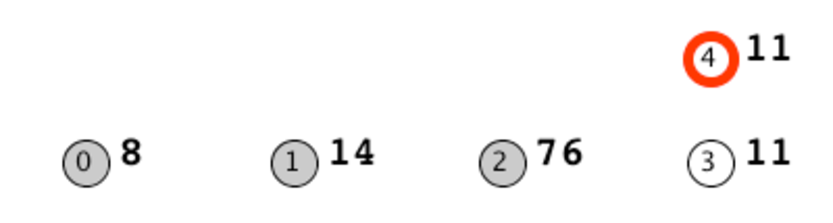
\includegraphics[scale=0.4]{X_is_1}
}

\smallskip
(a) Starting to insert \verb$x = A[3]$.

\bigskip
\fbox{
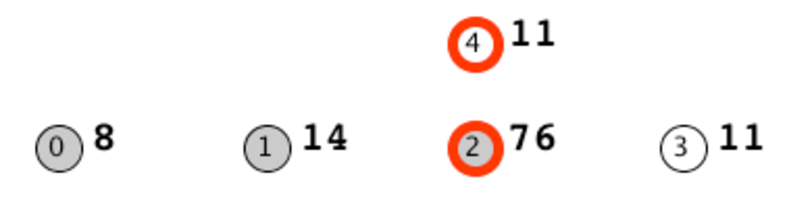
\includegraphics[scale=0.4]{X_is_2}
}

\smallskip
(b) Comparing \verb$x$ with \verb$A[2]$.

\bigskip
\fbox{
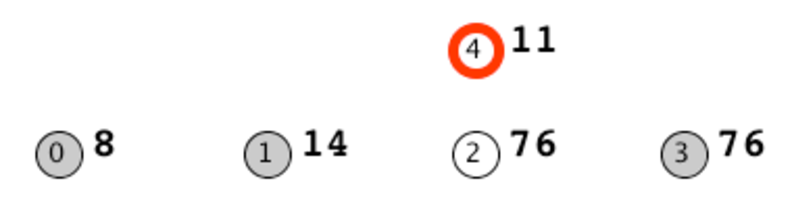
\includegraphics[scale=0.4]{X_is_3}
}

\smallskip
(c) \verb$A[2] > x$ so \verb$A[3] = A[2]$.

\end{center}

\caption{The insertion sort algorithm
and three steps in the animation.}
\label{fig:insertion_sort_animation}
\end{figure}


Fig.~\ref{fig:insertion_sort_animation}
illustrates an animation of insertion sort
that uses node movement and suggests that, with some creativity,
other sorting algorithms might be animated as well
-- this has already been done for bubble sort and merge sort.
At the beginning (not shown) the code:
(i)~puts nodes, evenly spaced, on a horizontal line;
(ii)~creates arrays \verb$nodes$, \verb$xCoord$ and \verb$A$, holding the
nodes, their horizontal positions and their weights (i.e., the array to be sorted), respectively; and (iii)~adds a new node \verb$toInsert$ for the
element to be inserted at each outer-loop iteration.

The rest of the code is a classic insertion sort implementation: nodes behave
as if they were array positions; those in the already sorted part of the array
are marked; a node that is being compared with \verb$x$ is highlighted.
To ensure this one-to-one correspondence between comparisons and highlighting,
there is a break in the middle of the main loop.
The first animation step highlights the two nodes being compared.
If the comparison signals that the loop should not be continued
a \texttt{break} statement causes an exit.
The second animation step then
(i)~copies the weight of \texttt{nodes[j]} (a.k.a. \texttt{A[j]})
to \texttt{nodes[j+1]};
(ii)~unhighlights \texttt{nodes[j]} to indicate that \texttt{A[j]} is no
longer involved in a comparison;
(iii)~unmarks \texttt{nodes[j]} to signal that \texttt{A[j]}
is in transition;
and (iv)~marks \texttt{nodes[j+1]} to indicate that \texttt{A[j+1]}
has its final value for this iteration of the outer loop.

The insertion sort animation begins with the declaration
\verb+movesNodes()+.
This prevents the user from moving nodes during algorithm execution.
Ordinarily, users \emph{are} allowed to change node positions during execution
to, for example, make labels and weights more visible.
The new positions persist after algorithm execution.
However, when an algorithm moves nodes, the nodes will revert to their original
positions when the algorithm is done.
Snapshots of positions (and other aspects of graph state)
during execution can be created using the
\textsf{Export} option on the file menu of the graph window.

